%! Author = phili
%! Date = 28/06/2021

\section{Bugs}
\textbf{Security Bug:}
\begin{itemize}
    \item Vulnerability at the implementation level
    \item Easy to discover / remediate using mondern code review tools
    \item E.g. buffer overflows, race conditions, unsafe system calls
\end{itemize}
\textbf{Security Flaw:}
\begin{itemize}
    \item Design level vulnerability
    \item Difficult / impossible to detect by automated tools
    \item Requires a manual risk analysis
    \item E.g. method overriding, error handling, type safety confusion
\end{itemize}
\textbf{Security Defect = Bug + Flaw}
\begin{itemize}
    \item Bugs / Flaws which may lie dormant for years
    \item Can surface in fielded systems with major consequences
\end{itemize}

\subsection{Example}
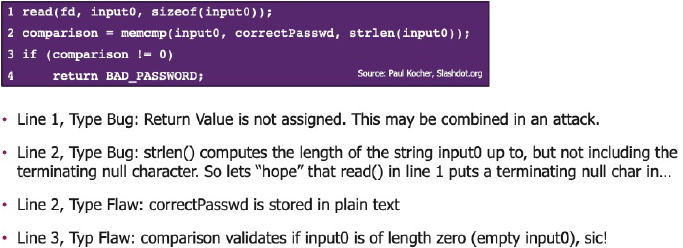
\includegraphics[width=\linewidth]{../img/bug_example.png}

\subsection{Memory Corruption}
\begin{itemize}
    \item Processes have their own address space others cant touch
    \item \textbf{Segmentation fault:} if a process tries to access memory outside its range
\end{itemize}

\subsubsection{Buffer Overflows}
\begin{lstlisting}
char buffer[4];
buffer[4] = 'a'; // Undefined behaviour
\end{lstlisting}
\begin{itemize}
    \item Can result in segmentation fault, if lucky
    \item Possible remote code execution, if unlucky
\end{itemize}
\textbf{Solution:}
\begin{itemize}
    \item Check array boundary at runtime
\end{itemize}

\subsubsection{Other memory corruption issues}
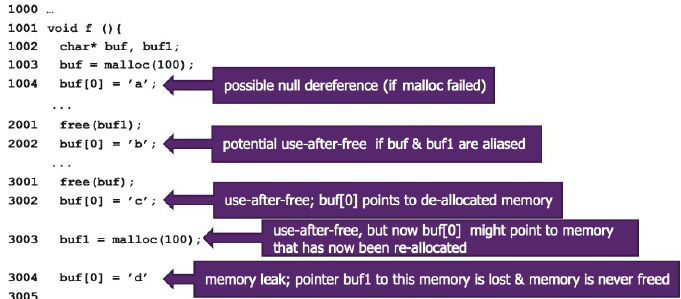
\includegraphics[width=\linewidth]{../img/memory_corruptions.png}

\subsection{Buffer Overflow}
\subsubsection{Process Memory Layout}
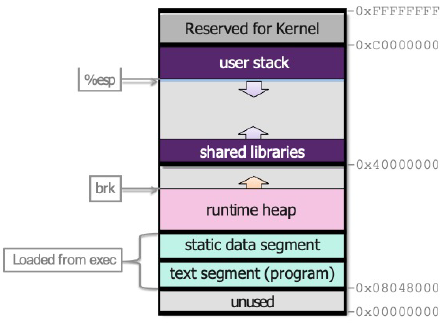
\includegraphics[width=0.6\linewidth]{../img/process_memory_layout.png}
\subsubsection{Stack Frame}
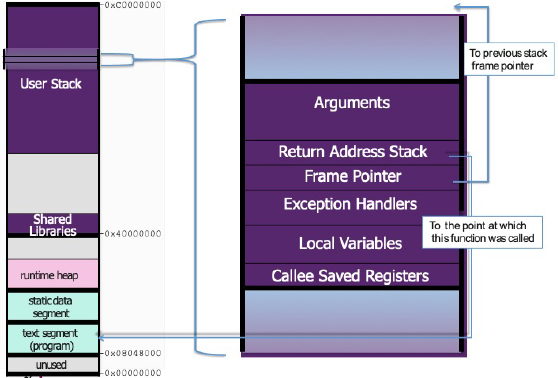
\includegraphics[width=0.6\linewidth]{../img/stack_frame.png}
\subsubsection{Problematic libc functions}
\begin{itemize}
    \item strcpy
    \item strcat
    \item gets
    \item scanf
\end{itemize}
\textbf{Safe versions:}
\begin{itemize}
    \item strncpy
    \item strncat
\end{itemize}

\subsubsection{Defenses}
\textbf{Compile:}\\
Harden programs to resist attacks in new programs.\\
\begin{itemize}
    \item Use a modern Programming Language
    \item Safe Coding Techniques
    \item Language Extensions / Safe Libraries
    \item Stack protection
    \begin{itemize}
        \item Canaries: Check function entry and exit code to check for corruption
        \item Random / Terminate canary
    \end{itemize}
\end{itemize}
\textbf{Run:}\\
Aim to detect and abort attacks in existing programs.\\
\begin{itemize}
    \item Executable Address Space Protection
    \begin{itemize}
        \item Use virtual memory support to make some regions of memory non-executable
    \end{itemize}
    \item ASLR: Address Space Layout Randomisation
    \item Non Executable Memory
\end{itemize}

\subsection{Race Condition}
\begin{itemize}
    \item Concurrency can lead to nondeterministic behaviour
    \item Software defects resulting from unanticipated execution ordering
    \item Necessary properties
    \begin{itemize}
        \item Concurrency
        \item Shared object
        \item Change state
    \end{itemize}
\end{itemize}

\subsubsection{Race Window}
\begin{itemize}
    \item Occurs in a code segment that accesses the race object
    \item Window of opportunity for race condition
    \item Critical Section
\end{itemize}

\subsubsection{Time of Check and Time of Use (ToCToU)}
\begin{itemize}
    \item Can occur during file I/O
    \item Forms a Race Window by first checking some race object and then using it
\end{itemize}
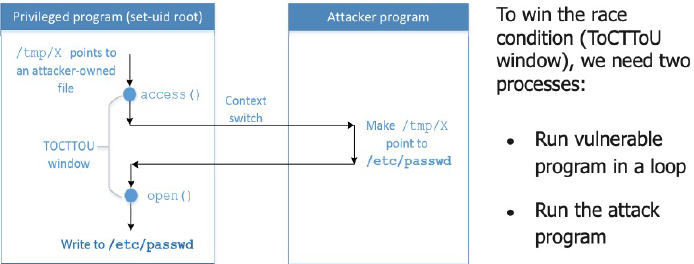
\includegraphics[width=\linewidth]{../img/toctou.png}

\subsubsection{How to Exploit Race Condition}
\begin{enumerate}
    \item Choose a target file (e.g. \textit{/etc/passwd})
    \item Launch Attack
    \begin{itemize}
        \item Attack Process
        \item Vulnerable Process
    \end{itemize}
    \item Monitor the result (check timestamp)
    \item Run the exploit
\end{enumerate}

\subsubsection{Mitigations}
\begin{itemize}
    \item Atomic Operations
    \item Repeating Check and Use
    \item Sticky Symlink Protection
    \item Principles of Least Privilege
\end{itemize}